% Chapter Template

\chapter{Graphical Models: Structural Modeling and Inference} % Main chapter title

\label{Chapter2} % Change X to a consecutive number; for referencing this chapter elsewhere, use \ref{ChapterX}

\lhead{Chapter 2. \emph{Graphical Models: Structural Modeling and Inference}} % Change X to a consecutive number; this is for the header on each page - perhaps a shortened title

\rule{\textwidth}{0.4pt} \\[0.5cm]
\textit{``Study the past if you would define the future."}

\begin{flushright}
Confucius
\end{flushright}
\rule{\textwidth}{0.4pt} 


Graphical models have been studied in many disciplines, such as artificial intelligence \citep{pearl_book}, statistics \citep{lauritzen_book} and communication \citep{MRF_communication}.  
Using graphical models is considered as one important landmark in machine learning research. Essentially, graphical models enable graphs to assist and facilitate probabilistic representation, 
analysis and computing. This chapter starts with two representative graphical models, \emph{Bayesian networks} and \emph{Markov networks} in section \ref{sec:PGMs}. Some fundamental basics, 
including \emph{factorizations, conditional independencies} and \emph{the conversions between Bayesian networks and Markov networks}, are explained. In section \ref{sec:inference}, three inference 
algorithms for graphical models are reviewed: \emph{(loopy) belief propagation}, \emph{variational methods} and \emph{Markov chain Monte Carlo} (MCMC). 
At last, an application of the modeling and inference with graphical models is presented in section \ref{sec:3D_Shape}, where a hybrid model,  
\emph{Spatial Latent Dirichlet Markov Random Fields}, is developed for learning 3D part-based shapes.             

The content in this chapter basically is a short summary of relevant materials collected from \cite{MLPR_book}, \cite{Barber_book}, \cite{Koller09} and \cite{Wainwright_book}.                   



%----------------------------------------------------------------------------------------
%	SECTION 1
%----------------------------------------------------------------------------------------
\section{Probabilistic Graphical Models}
\label{sec:PGMs}
Basically, graphical models are divided into two categories: directed and undirected ones. The most popular directed graphical model is \emph{Bayesian networks}, or \emph{Belief networks}; 
while the most widely used undirected graphical model is \emph{Markov networks}, or sometimes referred to as \emph{Markov random fields}. This section will cover both Bayesian networks and 
Markov networks by going through their basic properties.   

%-----------------------------------
%	SUBSECTION 1
%-----------------------------------
\subsection{Bayesian Networks}
Given a set of variables $\{x_1,x_2,\cdot, x_i\}$, one key function of graphical models is to model the interactions among them using graphs. A Bayesian network is a very 
intuitive graphical model by defining a joint distribution of  $\{x_1,x_2,\cdots, x_i\}$ with simple \emph{cause-effect} links. More precisely,  a Bayesian network is constructed by considering 
all cause-effect relations and linking them with directed arrows. Then the joint distribution can be factorized as the product of all conditional distributions associated with cause-effect relations. 
It is better to start with a real-world example \citep{Barber_book} for a 
quick understanding of the concept:   
\begin{shaded}
   \textbf{Wet-grass Example:} One morning Tracey found that the grass in her garden is wet ($T\in\{0,1\}$). Is it due to overnight rain ($R \in\{0,1\}$) or did
she forget to turn off the sprinkler last night ($S\in\{0,1\}$)? Next she notices that the grass of her neighbor, Jack, is also
wet ($J\in\{0,1\}$), and she also remembered it was cloudy on the previous daytime ($C\in\{0,1\}$).                   
\end{shaded}
In the above example, five binary variables are involved: $T,R,J,S,C$. After an easy analysis, the corresponding Bayesian network can be drawn as follows: 
\begin{figure}[h]
   \centering
   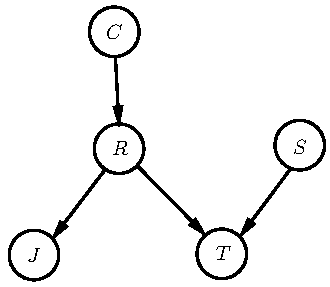
\includegraphics[width=0.4\textwidth]{./Figures/wet_glass_BN.pdf}
   \caption{The Bayesian network for the wet-grass example.}
\end{figure}

The joint distribution of these five variables is:
\begin{equation}
	P(J,T,R,C,S)=P(J|R)P(T|R,S)P(R|C)P(C)P(S)
	\label{equ:wet_grass}
\end{equation}
It is worth mentioning that the conditional distributions are definitely not limited to represent cause-effect relations.  
Actually, they are more often used to encode \emph{generation processes}. Therefore, Bayesian networks are usually 
used as generative models in many scenarios.  

A formal definition of a Bayesian network is given as:  
\begin{definition}
 A Bayesian network is a Directed Acyclic Graph (DAG), which corresponds to a distribution of the form:
 \begin{equation}
  P(X)=\prod_i P(x_i|\text{pa}(x_i))
 \end{equation}
where $X=\cup\{x_i\}$, pa$(x_i)$ denotes the parent nodes of $x_i$. 
\end{definition}

The \emph{factorization property} of the joint distribution of a Bayesian network is based on the \emph{conditional independencies} between variables. In the wet-grass example, some conditional 
indepencies can be figured out with common sense:
\begin{equation*}
\begin{array}{rcl}
 &&J\ci T|R, J\ci C|R, J\ci S|R\\
 &&T\ci C|R \\
 &&R\ci S|C \\
 &&C\ci S 
\end{array}
\end{equation*}
 

Meanwhile, a more systematic way to check conditinal independencies is \emph{D-separation rule}:   
\begin{theorem}
\textbf{D-Separation Rule}:
 Given three non-intersecting subsets of nodes $A,B,S$, in a DAG $G$, we consider all possible paths from any node in $A$ to any node in $B$. The path 
is said blocked if either: 
\begin{enumerate}
 \item the path goes through either \emph{head-to-tail} or \emph{tail-to-tail} at the node, and the node is in set $S$, or
 \item the path goes through \emph{head-to-head} at the node, and neither the node nor any of its descendants is in the set $S$. 
\end{enumerate}
If all paths are blocked, then S D-separates $A$ from $B$, and then:
\begin{equation*}
 A\ci B|S
\end{equation*}
\end{theorem}

The D-Separation rule can be empirically proved as follows:
\begin{proof}
	Three type of separating nodes: \emph{tail-to-tail}, \emph{head-to-tail} and \emph{head-to-head} are considered in three simple graphs respectively   \\ \\
	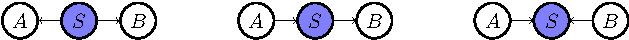
\includegraphics[width=\textwidth]{./Figures/D_Sep}\newline
\begin{minipage}[c]{0.32\textwidth}
 \begin{equation*}
  \begin{array}{rcl}
   & & P(A,B|S)\\
   &=& \frac{P(A,B,S)}{P(S)}\\
   &=& \frac{P(A|S)P(B|S)P(S)}{P(S)}\\
   &=& P(A|S)P(B|S)
  \end{array}
 \end{equation*}
\end{minipage}
\begin{minipage}[c]{0.32\textwidth}
 \begin{equation*}
  \begin{array}{rcl}
   & & P(A,B|S)\\
   &=& \frac{P(A,B,S)}{P(S)}\\
   &=& \frac{P(B|S)P(S|A)P(A)}{P(S)}\\
   &=& P(B|S)\frac{P(S|A)P(A)}{P(S)}\\
   &=& P(B|S)P(A|S)
  \end{array}
 \end{equation*}
\end{minipage}
\begin{minipage}[c]{0.32\textwidth}
 \begin{equation*}
  \begin{array}{rcl}
   & & P(A,B|S)\\
   &=& \frac{P(A,B,S)}{P(S)}\\
   &=& \frac{P(S|A,B)P(A)P(B)}{P(S)}\\
  \end{array}
 \end{equation*}
\end{minipage}\\
\end{proof}



%-----------------------------------
%	SUBSECTION 2
%-----------------------------------
\subsection{Markov Networks}
In a Bayesian network, the joint distribution is decomposed into (directed) conditional distributions. However, in many practical tasks, it is more interesting 
to model symmetric compatibility between two variables.           
A more general graph for modeling dependencies among variables is Markov networks, or sometimes referred to as Markov random fields (MRFs).      
To obtain a quick awareness of the modeling flexibility of Markov networks, it is helpful to rewrite the factorization of (\ref{equ:wet_grass}) as:    
\begin{equation}
 \begin{array}{rcl}
   & & P(J,T,R,C,S)\\
   &=& P(J|R)P(T|R,S)P(R|C)P(C)P(S) \\
   &=& \underbrace{P(J|R)}_{\phi_1(J,R)} \underbrace{P(R|C)P(C)}_{\phi_2(R,C)} \underbrace{P(T|R,S)P(S)}_{\phi_3(T,R,S)}\\
   &=& \phi_1(J,R)\phi_2(R,C)\phi_3(T,R,S)
 \end{array}
 \label{equ:BN2MN}
\end{equation}
where $\phi_1(J,R), \phi_2(R,C),\phi_3(T,R,S)$ are no longer conditional probabilities. As a matter of fact, in Markov netowrks, 
$\phi_1(J,R), \phi_2(R,C),\phi_3(T,R,S)$ even 
do not have to be distributions. They can be compatibilities represented by any parametric form. Meanwhile, since $P(J,T,R,C,S)$ is still a distribution, 
\emph{i.e.} $\sum_{J,T,R,C,S}P(J,T,R,C,S)=1$, a normalization needs to be introduced.   

A formal definition of a Markov network is given as follows: 
\begin{definition}
 A Markov Network is an undirected graph which corresponds to the distribution of the form:
 \begin{equation}
  P(x_1,x_2,...x_n)=\frac{1}{Z}\prod_{c}\phi_c(X_c)
  \label{equ:MN_factorization}
 \end{equation}
 where $X_c$ is a \emph{clique} of the graph nodes, and $\phi_c(X_c)$ is called \emph{potential function} over clique $X_c$, and $Z$ is to ensure the distribution normalized.
\end{definition}
\textbf{Remarks:}
\begin{itemize}
 \item the potential function is non-negative, and can be a function of any form over the clique $X_c$, and in most cases it reflects the dependences /compatibilities /constrains among $x_i\in X_c$ ;
 \item the normalization term can be computed as $Z=\sum_{x_1,x_2,\dots,x_n}\prod_{c}\phi_c(X_c)$ or $Z=\int_{x_1,x_2,\dots,x_n}\prod_{c}\phi_c(X_c)$ for continuous cases;
 \item the clique defined here means maximal \emph{fully connected subgraph}, some examples of cliques and potential functions are shown in the following: 
\end{itemize}
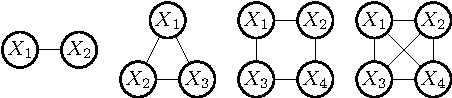
\includegraphics[width=\textwidth]{./Figures/clique}\newline
\begin{minipage}[c]{0.24\textwidth}
 \begin{equation*}
  \psi(X_1,X_2)
 \end{equation*}
\end{minipage}
\begin{minipage}[c]{0.24\textwidth}
 \begin{equation*}
  \psi(X_1,X_2,X_3)
 \end{equation*}
\end{minipage}
\begin{minipage}[c]{0.25\textwidth}
 \begin{equation*}
  \begin{array}{rcl}
   && \psi(X_1,X_2)\\
   && \psi(X_2,X_4)\\
   && \psi(X_1,X_3)\\
   && \psi(X_3,X_4)
  \end{array}
 \end{equation*}
\end{minipage}
\begin{minipage}[c]{0.24\textwidth}
 \begin{equation*}
 \psi(X_1,X_2,X_3,X_4)
 \end{equation*}
\end{minipage}

Similarly to Bayesian networks, the factorization of (\ref{equ:MN_factorization}) is also based on the conditional independencies among variables.      
Meanwhile, in Markov networks, checking conditional independencies is much simpler than D-separation rule. The rule for checking  conditional independencies 
in Markov networks is referred to as \emph{Markov separation rule}:
\begin{theorem}
\textbf{Markov Separation Rule} : a subset $\mathcal{A}$ is said to be separated from another subset $\mathcal{B}$ 
by subset $\mathcal{S}$ if all possible paths from any member of $\mathcal{A}$ to any member $\mathcal{B}$
pass through $\mathcal{S}$. If $\mathcal{S}$ separates $\mathcal{A}$ from $\mathcal{B}$, then
 \begin{equation*}
 \mathcal{A} \ci \mathcal{B} | \mathcal{S}
  \end{equation*}
\end{theorem}
The equivalence between the factorization of Markov networks and Markov separation rule is proved in \emph{Hammersley-Clifford theorem} \citep{HC_theorem}.  


Based on the Markov separation rule, several interesting and useful properties can be further derived.   
\begin{corollary}
\textbf{Local Conditional Independence}:
  when conditioned on its neighbors, $x_i$ is  independent of all other variables of the graph: 
   \begin{equation*}
    P(x_i|X \backslash x_i)= P(x_i|\text{ne}(x_i))
   \end{equation*}
\end{corollary}
For instance, \newline\newline 
\begin{minipage}[c]{0.5\textwidth}   
	\centering
	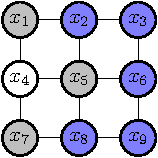
\includegraphics[width=0.5\textwidth]{./Figures/markov_net_1.pdf}
\end{minipage}
\begin{minipage}[c]{0.5\textwidth}
   \begin{equation*}
 \Longrightarrow x_4 \ci \{x_2,x_3,x_6,x_8,x_9 \}|\{x_1,x_5,x_7\}
   \end{equation*}
\end{minipage}
\newline 

\begin{corollary}
\textbf{Pairwise Conditional Independence}:
  given two non-adjacent variables $x_i$ and $x_j$, they are independent conditioned on all other variables of the graph:
 \begin{equation*}
  x_i \ci x_j | X \backslash \{x_i,x_j\}
 \end{equation*}
\end{corollary}
For instance,  \newline\newline 
\begin{minipage}[c]{0.5\textwidth}   
	\centering
	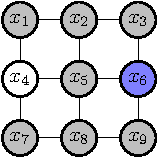
\includegraphics[width=0.5\textwidth]{./Figures/markov_net_2.pdf}
\end{minipage}
\begin{minipage}[c]{0.4\textwidth}
   \begin{equation*}
  \Longrightarrow  x_4 \ci x_6 |\{x_1,x_2,x_3,x_5,x_7,x_8,x_9\}
   \end{equation*}
\end{minipage}


%-----------------------------------
%	SUBSECTION 3
%-----------------------------------
\subsection{Connecting Bayesian Networks and Markov Networks}
As shown in (\ref{equ:BN2MN}), a Bayesian network can be also considered as a Markov network which uses conditional distributions 
as its potential functions. However, the corresponding graph also needs to be modified to fit the conditional independencies and Markov separation 
rule. The modification procedure is:        
\begin{enumerate}
	\item find all parents which share a common child and connect them with undirected links;   
	\item remove all arrows in the graph.     
\end{enumerate}
The first step is usually called ``moralization" since it binds unconnected parents together. For example, converting the Bayesian network of 
the wet-grass example to a Markov network is shown in Figure \ref{fig:BN_2_MN}.    
\begin{figure}
	\subfigure[]{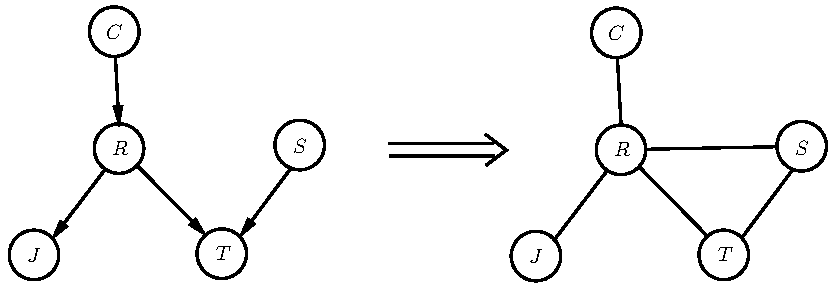
\includegraphics[width=0.65\textwidth]{./Figures/BN_2_MN.pdf}{\label{fig:BN_2_MN}}}\quad \quad \quad
	\subfigure[]{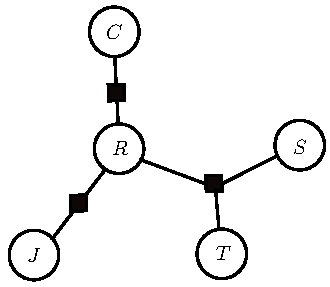
\includegraphics[width=0.26\textwidth]{./Figures/factor_graph.pdf}{\label{fig:factor_graph}}}
	\caption{(a) Converting the Bayesian network of 
	the wet-grass example to a Markov network; (b) the factor graph the wet-grass example. }
\end{figure}

Conversion from Markov networks to Bayesian networks is also possible by using \emph{Chordal graphs}. However, the procedure is more complicated 
and seldom used.  Another way for connecting Bayesian networks and Markov networks is using \emph{factor graphs}, which is also an undirected graphical model. 
However, \emph{factor nodes} (usually represented by solid squares) are used in factor graphs to encode interactions. Therefor, the specifications of cliques  
in Markov networks, or conditional distributions in Bayesian networks, are no more necessary. A factor graph of the wet-grass example is shown in Figure \ref{fig:factor_graph}.      



%----------------------------------------------------------------------------------------
%	SECTION 2
%----------------------------------------------------------------------------------------
\section{Exact and Approximate Inference}
\label{sec:inference}
It has been shown that how Bayesian networks or Markov network can be used for modeling dependencies among multiple variables. Meanwhile, a more practically important 
function of graphical models is that inference tasks can be facilitated by exploiting graph properties.           
As studied in the previous section, Bayesian networks can be easily converted to Markov networks. Therefore, in this section, the inference algorithms are explained based on 
Markov network cases.   
%-----------------------------------
%	SUBSECTION 1
%-----------------------------------
\subsection{Belief Propagation}
A main inference task is computing marginal distributions, based on which conditional distributions can be subsequently computed as well.    
Again, an example is first illustrated to understand the procedure of computing marginal distributions, based on which the \emph{belief propagation} algorithm will be explained  
later. 

In a tree-structured Markov network shown below, $A,B,C,D$ are four variables and each of them has $n$ states. Then how to compute $P(A)$ ?
\newline 
\begin{minipage}[c]{0.4\textwidth}
      \centering
      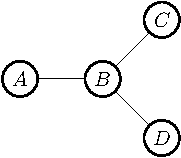
\includegraphics[width=0.75\textwidth]{./Figures/message_passing}
\end{minipage}
\begin{minipage}[c]{0.6\textwidth}
 \begin{equation*}
  \begin{array}{rcl}
  & & P(A) \\
  &=& \overbrace{\sum_{B,C,D}P(A,B,C,D)}^{complexity:  \mathcal{O}(n^{3})} \\
  &\propto& \sum_{B,C,D} \left[ \phi(A,B) \phi(B,C) \phi(B,D) \right] \\
  &\propto& \sum_{B}\phi(A,B) \underbrace{\sum_C \phi(B,C)}_{m_{C\rightarrow B}(B)} \underbrace{\sum_D \phi(B,D)}_{m_{D\rightarrow B}(B)}\\ 
  &\propto& \sum_{B} \left\{\phi(A,B) m_{C\rightarrow B}(B) m_{D\rightarrow B}(B) \right\} \\
  &\propto& m_{B\rightarrow A}(A)
  \end{array}
 \end{equation*}
\end{minipage}
\newline 

In the above procedure, it can be seen that the computation complexity of calculating $p(A)$ is in general $\mathcal{O}(n^3)$. However, by exploiting 
the graph structure and corresponding factorization, the complexity is reduced to $O(n)$. Basically, a new ``message function" $m(\cdot)$ is introduced; 
each variable is eliminated by first summing 
itself up in the product of potential functions and $m$ functions which involves it, and then passing a marginalize message to its neighbouring variable. 
This procedure is repeatedly carried out 
on all variables until it reaches $A$. To demonstrate the ``message-passing" theme more clearly,  messages and passing directions are added in the Markov networks and  
highlighted below:
\newline
\begin{minipage}[c]{0.4\textwidth}
      \centering
      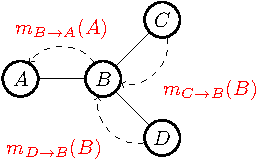
\includegraphics[width=1.1\textwidth]{./Figures/message_passing_1}
\end{minipage}
\begin{minipage}[c]{0.6\textwidth}
 \begin{equation*}
  \begin{array}{rcl}
  & & P(A) \\
  &\propto& \sum_{B}\phi(A,B) \sum_C \phi(B,C) \sum_D \phi(B,D)\\ 
  &\propto& \sum_{B} \left\{\phi(A,B) m_{C\rightarrow B}(B) m_{D\rightarrow B}(B) \right\} \\
  &\propto& m_{B\rightarrow A}(A)
  \end{array}
 \end{equation*}
\end{minipage}\\
\newline 
\textbf{Remarks:}
$m_{C\rightarrow B}(B)$ is called \emph{belief function} of $B$ over $C$ by summing out $C$ from the potential function $\sum_C \phi(B,C)$, and it will propagate afterwards; 

Similarly, $P(C)$ can be computed with the propagations of belief functions: 
\newline
\begin{minipage}[c]{0.4\textwidth}
      \centering
      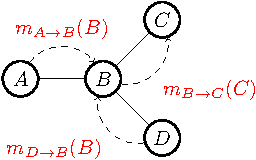
\includegraphics[width=1.1\textwidth]{./Figures/message_passing_2}
\end{minipage}
\begin{minipage}[c]{0.6\textwidth}
 \begin{equation*}
  \begin{array}{rcl}
  & & P(C) \\
  &\propto& \sum_{A}\phi(A,B) \sum_B \phi(B,C) \sum_D \phi(B,D)\\ 
  &\propto& \sum_B \phi(B,C)  \sum_{A}\phi(A,B) \sum_D \phi(B,D)\\ 
  &\propto& \sum_{B} \left\{   \phi(B,C) m_{A\rightarrow B}(B) m_{D\rightarrow B}(B) \right\} \\
  &\propto& m_{B\rightarrow C}(C)
  \end{array}
 \end{equation*}
\end{minipage}
\newline 
\newline 
\newline 
and $P(B)$ as well:
\newline 
\newline 
\begin{minipage}[c]{0.4\textwidth}
      \centering
      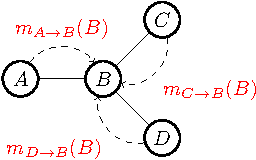
\includegraphics[width=1.1\textwidth]{./Figures/message_passing_3}
\end{minipage}
\begin{minipage}[c]{0.6\textwidth}
 \begin{equation*}
  \begin{array}{rcl}
  & & P(B) \\
  &\propto& \sum_{A}\phi(A,B) \sum_C \phi(B,C) \sum_D \phi(B,D)\\  
  &\propto& m_{A\rightarrow B}(B) m_{C\rightarrow B} (B) m_{D\rightarrow B}(B)  \\
  \end{array}
 \end{equation*}
\end{minipage}\\

Based on three examples above, some observations of ``message passing" are:  
\begin{itemize}
	\item  one variable can send a message to one of its neighbor only if it has received messages from all other variables  

  \begin{equation*}
   m_{B\rightarrow C}(C)=\sum_{B} \left\{   \phi(B,C) m_{A\rightarrow B}(B) m_{D\rightarrow B}(B) \right\}
  \end{equation*}

 \item marginal probabilities are computed as the product of incoming messages:
  \begin{equation*}
  \begin{array}{rcl}
   P(B)&=&\frac{1}{Z}m_{A\rightarrow B}(B) m_{C\rightarrow B} (B) m_{D\rightarrow B}(B)\\
   P(A)&=&\frac{1}{Z}m_{B\rightarrow A}(A) \\
   P(C)&=&\frac{1}{Z}m_{B\rightarrow C}(C) \\
   P(D)&=&\frac{1}{Z}m_{B\rightarrow D}(D) 
  \end{array}
 \end{equation*}
 \item messages are asymmetric and thus associated with directions;       
 \item messages are reused in many inference tasks, therefore it is more efficient to compute all messages first and 
	 then conduct inference. 
\end{itemize}

Based on the observations above, the belief propagation algorithm for tree-structured Markov networks can be written out in Algorithm \ref{alg:BP_tree}.       
\begin{algorithm}
	\caption{Belief Propagation for tree-structured Markov networks}
	\label{alg:BP_tree}
\begin{algorithmic}[1]
\STATE  select one variable as the root; 
\STATE  starting from all leaves, propagate \emph{beliefs} toward the root as:
\begin{equation*}
m_{i \rightarrow j}(x_j)= \sum_{x_i}\left\{\phi(x_i,x_j) \prod_{k\in \text{Ne}(i)\backslash j} m_{k \rightarrow i}(x_i)\right\}
\end{equation*}
\STATE  when the root receives all messages from its neighbors, then propagate backwards the \emph{``inverse beliefs"} as the step 2;
\STATE  the marginal probability of each variable is computed as: 
\begin{equation*}
P(x_i)\propto \prod_{k\in \text{Ne}(i)} m_{k \rightarrow i}(x_i)
\end{equation*}
where Ne$(i)$ denotes the neighboring variables of $x_i$ in the graph. 
\end{algorithmic}
\end{algorithm}


However, in grid-structured Markov networks, there is no root and leaves, where the belief propagation algorithm can not be directly applied.  
Fortunately, an approximate version of the belief propagation algorithm, \emph{loopy belief propagation}, was proposed for the inference of 
loopy Markov networks. Basically, in the loop belief propagation algorithm, all messages are randomly initialized and iteratively updated based on 
the same passing rules as in the belief propagation algorithm.   A pseudo-code of the loopy belief propagation algorithm is presented in Algorithm \ref{alg:LBP}.     
Until now, there exist no theoretic proof for the convergence the loopy belief propagation algorithm. However, it has been applied in many tasks 
and empirically works well.  
\begin{algorithm}
	\caption{Loopy Belief Propagation for Loopy Markov networks}
	\label{alg:LBP}
\begin{algorithmic}[1]
%\STATE  In a loopy graph, there is no root and leaves because of loop.
\STATE  initialize all messages $m_{i\rightarrow j}$ in both directions of all connected variables randomly or with a constant value (\emph{e.g.} 1);
\WHILE {all messages converge}
\STATE  update messages as:
\begin{equation*}
  m^{(t+1)}_{i \rightarrow j}(x_j)= \sum_{x_i}\left\{\phi(x_i,x_j) \prod_{k\in \text{Ne}(i)\backslash j} m^{(t)}_{k \rightarrow i}(x_i)\right\}
\end{equation*}
\ENDWHILE
\end{algorithmic}
\end{algorithm}

%-----------------------------------
%	SUBSECTION 2
%-----------------------------------
\subsection{Markov Chain Monte Carlo}
Another way for approximate inference is using samples and \emph{Monte-Carlo estimations}.      
Markov chain Monte Carlo (MCMC) is a very general and powerful framework for sampling. In particular, Gibbs sampling is popularly used in Markov networks.    
MCMC is a family of sampling algorithms, which are designed to generate samples from a target distribution $p(\mathbf{x}), \mathbf{x}\in\mathbb{R}^d$. 
Usually, directly sampling from $p(\mathbf{x})$ is not possible since its density can be arbitrarily complex. However, $p(\mathbf{x})$ can be evaluated up to a normalizing constant, \emph{e.g.} a 
Markov network:
\begin{equation*}
	p(\mathbf{x})=\frac{\tilde{p}(\mathbf{x})}{\mathbf{Z}}
\end{equation*}
%The target distribution $p(\mathbf{x})$ can be marginal distributions or conditional distributions based on the inference task.      

A Markov chain of $\mathbf{x}$ is specified by a \emph{transition probability}, based on which the state of $\mathbf{x}$ can 
be evolved. The transition probability defines how the state of $\mathbf{x}$ at the current step changes to the next step: $\mathcal{T}(\mathbf{x}^{t+1}|\mathbf{x}^t)$.      
The distribution $p(\mathbf{x})$ is said to be \emph{invariant} with respect to a Markov chain with the transition  $\mathcal{T}(\mathbf{x}^{t+1}|\mathbf{x}^t)$ if
\begin{equation}
	p(\mathbf{x}^*)=\sum_{\mathbf{x}^t}\mathcal{T}(\mathbf{x}^*|\mathbf{x}^t)p(\mathbf{x}^t)
\end{equation}
A sufficient (but not necessary) condition for checking whether $p(\mathbf{x})$ is invariant with respect to the Markov chain with $\mathcal{T}$ is \emph{detailed balance}:
\begin{equation}
  p(\mathbf{x}^t) \mathcal{T}(\mathbf{x}^*|\mathbf{x}^t)=p(\mathbf{x}^*) \mathcal{T}(\mathbf{x}^t|\mathbf{x}^*)
\end{equation}
\subsubsection{Metropolis Algorithm}
The \emph{Metropolis algorithm} is the simplest MCMC sampling method. The transition probability in the Metropolis algorithm is specified by a \emph{proposal distribution} and 
an \emph{acceptance probability}:
\begin{itemize}
	\item the proposal distribution is symmetric: $q(\mathbf{x}^*|\mathbf{x}^t)=q(\mathbf{x}^t|\mathbf{x}^*)$;
	\item the acceptance probability is: $\mathcal{A}(\mathbf{x}^*;\mathbf{x}^t) = \min\{1, \frac{p(\mathbf{x}^*)}{p(\mathbf{x}^t)}\}$; 
\end{itemize}
A pseudo-code of the Metropolis algorithms is provided in Algorithm \ref{alg:Metropolis}.  
It can be seen in the Metropolis algorithm that  $\mathbf{x}^0,\mathbf{x}^1,\cdots, \mathbf{x}^t$ are not independent because successive samples are correlated. Therefore, in practice, real independent 
samples can be obtained by only retraining samples at every $M$ iterations. 
    

The detailed balance of the Metropolis algorithm can be proved as follows:
\begin{proof}
	\begin{equation}
		\begin{array}{rcl}
			p(\mathbf{x}^t)\mathcal{T}(\mathbf{x}^*|\mathbf{x}^t)&=&p(\mathbf{x}^t)\left(q(\mathbf{x}^*|\mathbf{x}^t)\min\{1,\frac{p(\mathbf{x}^*)}{p(\mathbf{x}^t)}\}\right) \\
												       &=& \min\{p(\mathbf{x}^t)q(\mathbf{x}^*|\mathbf{x}^t),q(\mathbf{x}^*|\mathbf{x}^t)p(\mathbf{x}^*) \}  \\
			                                           &=&p(\mathbf{x}^*)q(\mathbf{x}^*|\mathbf{x}^t)\min\{1,\frac{p(\mathbf{x}^t)}{p(\mathbf{x}^*)}\} \\
																											 &\overset{\text{since } q(\mathbf{x}^*|\mathbf{x}^t)=q(\mathbf{x}^t|\mathbf{x}^*)}=& p(\mathbf{x}^*)\left(q(\mathbf{x}^t|\mathbf{x}^*) \min\{1,\frac{p(\mathbf{x}^t)}{p(\mathbf{x}^*)}\} \right) \\
																									&=& p(\mathbf{x}^*)\mathcal{T}(\mathbf{x}^t|\mathbf{x}^*)
	   \end{array}
	\end{equation}
\end{proof}

\begin{algorithm}[h]
	\caption{Metropolis Algorithm}
	\label{alg:Metropolis}
\begin{algorithmic}[1]
\STATE initialize $\mathbf{x}^0$.
\FOR {$t=0$ to $T-1$}
\STATE generate a sample uniformly from $[0,1]$: $u\sim \mathcal{U}_{[0,1]}$.
\STATE generate a sample from a symmetric proposal distribution: $\mathbf{x}^*\sim q(\mathbf{x}^*|\mathbf{x}^t)$.
\IF {$u<\min\{1,\frac{p(\mathbf{x}^*)}{p(\mathbf{x}^t)}\}$}
\STATE $\mathbf{x}^{t+1}=\mathbf{x}^*$.
\ELSE 
\STATE $\mathbf{x}^{t+1}=\mathbf{x}^t$.
\ENDIF
\ENDFOR
\end{algorithmic}
\end{algorithm}

\subsubsection{Metropolis-Hastings Algorithm} 
In the Metropolis algorithm, the proposal distribution is restricted to be symmetric, which limits its applicabilities.   A more general extension is the \emph{Metropolis-Hastings algorithm}, 
of which the proposal distribution and the acceptance probability are specified as follows:
\begin{itemize}
	\item the proposal distribution can be arbitrary (no symmetric restriction): $q(\mathbf{x}^*|\mathbf{x}^t)$;
	\item the acceptance probability is: $\mathcal{A}(\mathbf{x}^*;\mathbf{x}^t) = \min\{1, \frac{p(\mathbf{x}^*)q(\mathbf{x}^t|\mathbf{x}^*)}{p(\mathbf{x}^t)q(\mathbf{x}^*|\mathbf{x}^t)}\}$; 
\end{itemize}
The pseudo-code of the Metropolis-Hastings algorithm is presented in Algorithm \ref{alg:MH}. 
The detailed balance of the Metropolis algorithm can be proved as follows:
\begin{proof}
	\begin{equation}
		\begin{array}{rcl}
			p(\mathbf{x}^t)\mathcal{T}(\mathbf{x}^*|\mathbf{x}^t)&=&p(\mathbf{x}^t)\left(q(\mathbf{x}^*|\mathbf{x}^t)\min\{1,\frac{p(\mathbf{x}^*)q(\mathbf{x}^t|\mathbf{x}^*)}{p(\mathbf{x}^t)q(\mathbf{x}^*|\mathbf{x}^t)}\}\right) \\
												       &=& \min\{p(\mathbf{x}^t)q(\mathbf{x}^*|\mathbf{x}^t),q(\mathbf{x}^*|\mathbf{x}^t)p(\mathbf{x}^*) \}  \\
			                                           &=& p(\mathbf{x}^*)q(\mathbf{x}^t|\mathbf{x}^*)\min\{1,\frac{p(\mathbf{x}^t)q(\mathbf{x}^*|\mathbf{x}^t)}{p(\mathbf{x}^*)q(\mathbf{x}^t|\mathbf{x}^*)}\} \\
										&=& p(\mathbf{x}^*)\left(q(\mathbf{x}^t|\mathbf{x}^*)\min\{1,\frac{p(\mathbf{x}^t)q(\mathbf{x}^*|\mathbf{x}^t)}{p(\mathbf{x}^*)q(\mathbf{x}^t|\mathbf{x}^*)}\}\right) \\
											  &=& p(\mathbf{x}^*)\mathcal{T}(\mathbf{x}^t|\mathbf{x}^*)
	   \end{array}
	\end{equation}
\end{proof}
\begin{algorithm}[h]
	\caption{Metropolis-Hastings (MH) Algorithm}
	\label{alg:MH}
\begin{algorithmic}[1]
\STATE initialize $\mathbf{x}^0$.
\FOR {$t=0$ to $T-1$}
\STATE generate a sample uniformly from $[0,1]$: $u\sim \mathcal{U}_{[0,1]}$.
\STATE generate a sample $\mathbf{x}^*\sim q(\mathbf{x}^*|\mathbf{x}^t)$.
\IF {$u<\min\{1,\frac{p(\mathbf{x}^*)q(\mathbf{x}^t|\mathbf{x}^*)}{p(\mathbf{x}^t)q(\mathbf{x}^*|\mathbf{x}^t)}$}
\STATE $\mathbf{x}^{t+1}=\mathbf{x}^*$.
\ELSE 
\STATE $\mathbf{x}^{t+1}=\mathbf{x}^t$.
\ENDIF
\ENDFOR
\end{algorithmic}
\end{algorithm}





\subsubsection{Gibbs Sampling Algorithm}
Gibbs sampling is a special case of Me with the cyclic conditional distributions among $\{x_1,x_2,\cdots,x_d\}$ as the proposal distribution. Therefore,  
\begin{itemize}
	\item the proposal distribution: $q(\mathbf{x}^*|\mathbf{x}^t)=p(x_k^*|x_{[1,\cdots,d]/k}^t)$;
	\item the acceptance probability is: 
		\begin{equation*}
			\begin{array}{rcl}
				\mathcal{A}(\mathbf{x}^*;\mathbf{x}^t) &=& \min\left\{1, \frac{p(\mathbf{x}^*)q(\mathbf{x}^t|\mathbf{x}^*)}{p(\mathbf{x}^t)q(\mathbf{x}^*|\mathbf{x}^t)}\right\} \\
																				  &=& \min\left\{1, \frac{p(\mathbf{x}^*)p(x_k^t|x_{[1,\cdots,d]/k}^*)}{p(\mathbf{x}^t)p(x_k^*|x_{[1,\cdots,d]/k}^t)}\right\} \\
																			   &=& \min\left\{1,\frac{p(x_{[1,\cdots,d]/k}^*)p(x_k^*|x^*_{[1,\cdots,d]/k})p(x_k^t|x_{[1,\cdots,d]/k}^*)}{p(x^t_{[1,\cdots,d]/k})p(x_k^t|x^t_{[1,\cdots,d/k]})p(x_k^*|x_{[1,\cdots,d]/k}^t)} \right \} \\
											  &\overset{\text{since }x_{[1,\cdots,d]/k}^*=x_{[1,\cdots,d]/k}^t}=& \min\{1,1\} \\
							   &=&1
        	\end{array}
	    \end{equation*}
\end{itemize}
Obviously,  the proposal at each iteration is accepted in Gibbs sampling. The pseudo-code of Gibbs sampling is given in Algorithm \ref{alg:gibbs}.    
\begin{algorithm}[h]
	\caption{Gibbs Sampling Algorithm}
	\label{alg:gibbs}
\begin{algorithmic}[1]
\STATE initialize $\mathbf{x}^0$.
\FOR {$t=0$ to $T-1$}
\STATE randomly select   
\STATE sample $x^*_k$ from  $p(x_k^*|x_{[1,\cdots,d]/k}^t)$.
\STATE $x^{t+1}_k=x^*_k$.
\ENDFOR
\end{algorithmic}
\end{algorithm}

%-----------------------------------
%	SUBSECTION 3
%-----------------------------------
\subsection{Variational Methods}
Variational methods are an alternative to sampling-based methods for approximate inference. Basically, variational methods convert the inference problem into a constrained optimization 
problem, where standard optimization tools can be applied. For instance, to approximate a distribution $p(\mathbf{x})$, a family of distributions $q(\mathbf{x})$ is used and the optimal 
one is eventually selected by using certain optimization machinery. In a Markov network $p(\mathbf{x})$, the \emph{energy} is defined as: 
\begin{equation}
	E(\mathbf{x})=-\log p(\mathbf{x})-\log Z
\end{equation}
and the \emph{variational free energy} with $q(\mathbf{x})$ is defined as: 
\begin{equation}
	\begin{array}{rcl}	
	F(q)&=&\displaystyle\sum_{\mathbf{x}}q(\mathbf{x}) E(\mathbf{x})+\sum_{\mathbf{x}}\log q(\mathbf{x})\\ 
	\displaystyle		   &=&\underbrace{-\sum_{\mathbf{x}}q(\mathbf{x})\log p(\mathbf{x})+\sum_{\mathbf{x}} q(\mathbf{x})\log q(\mathbf{x})}_{KL(q(\mathbf{x}),p(\mathbf{x}))}-\log Z
    \end{array}
\end{equation}
It can be seen that the variational free energy can be minimized when $q(\mathbf{x})=p(\mathbf{x})$. Therefore, the joint distribution $p(\mathbf{x})$ is considered as 
the optimal solution in the optimization problem: $\arg\min_{q} F(q)$.  

The simplest variation method is the \emph{mean field} approximation, where $q(\mathbf{x})$ is a locally factorized: $q(\mathbf{x})=\prod_{i}q_i(x_i)$. Then the variational free energy is: 
\begin{equation}
	F_{MF}(q)=-\sum_{c}\sum_{\mathbf{x}_c}\log \phi_c(\mathbf{x}_c) \prod_{i\in c}q_i (x_i)+ \sum_i\sum_{x_i} q_i(x_i)\log q_i(x_i)
\end{equation}
where $c$ indexes cliques. Then the approximate marginal distribution of each variable $q_i(x_i)$ is updated according to:    
\begin{equation}
	q_i(x_i)=\alpha \exp \left(\sum_{c\in\mathcal{C}_i} \sum_{\mathbf{x}_{c/i}} \log \phi_c(\mathbf{x}_c)\prod_{j\in c, j\neq i}q_j(x_j)\right)
\end{equation}
where $\mathcal{C}_i$ denotes the set of all cliques which $x_i$ occupies and $\alpha$ is a normalization term for $\sum_{x_i}q_i (x_i)=1$.   

%----------------------------------------------------------------------------------------
%	SECTION 3
%----------------------------------------------------------------------------------------
\section{3D Part-Based Shape Modeling with Spatial Latent Dirichlet Markov Random Fields}
\label{sec:3D_Shape}
This section presents an application of graphical models on 3D part-based shape modeling. In particular, to fit the target of the task and make full use of various heuristics, 
both Bayesian networks and Markov networks are utilized. On the one hand, it is desired to have shape generative models, which can capture the composition processes of parts        
in different shapes. On the other hand, local and global spatial coherences need to be taken into account when conducting segmentation.  
Therefore, a hybrid model, \emph{spatial latent Dirichlet Markov random fileds}, is developed by integrating \emph{latent Dirichlet allocation} (LDA), \emph{mixture of Gaussians} (MoGs) and  
a Markov random field. In addition, Gibbs sampling is applied for inference in the hybrid model.      
More technical details and results are presented in the paper VI by the author. 

\begin{shaded}
{\Huge VI.} \textbf{Hanchen Xiong}, Sandor Szedmak, Justus Piater. {\it 3D Object Class Geometry Modeling with Spatial Latent Dirichlet Markov Random Fields}, In Proceedings of the 35th German Conference on Pattern Recognition (GCPR13), pp 51-60, 2013,  Springer.  
\vspace{-.2cm}

\end{shaded}
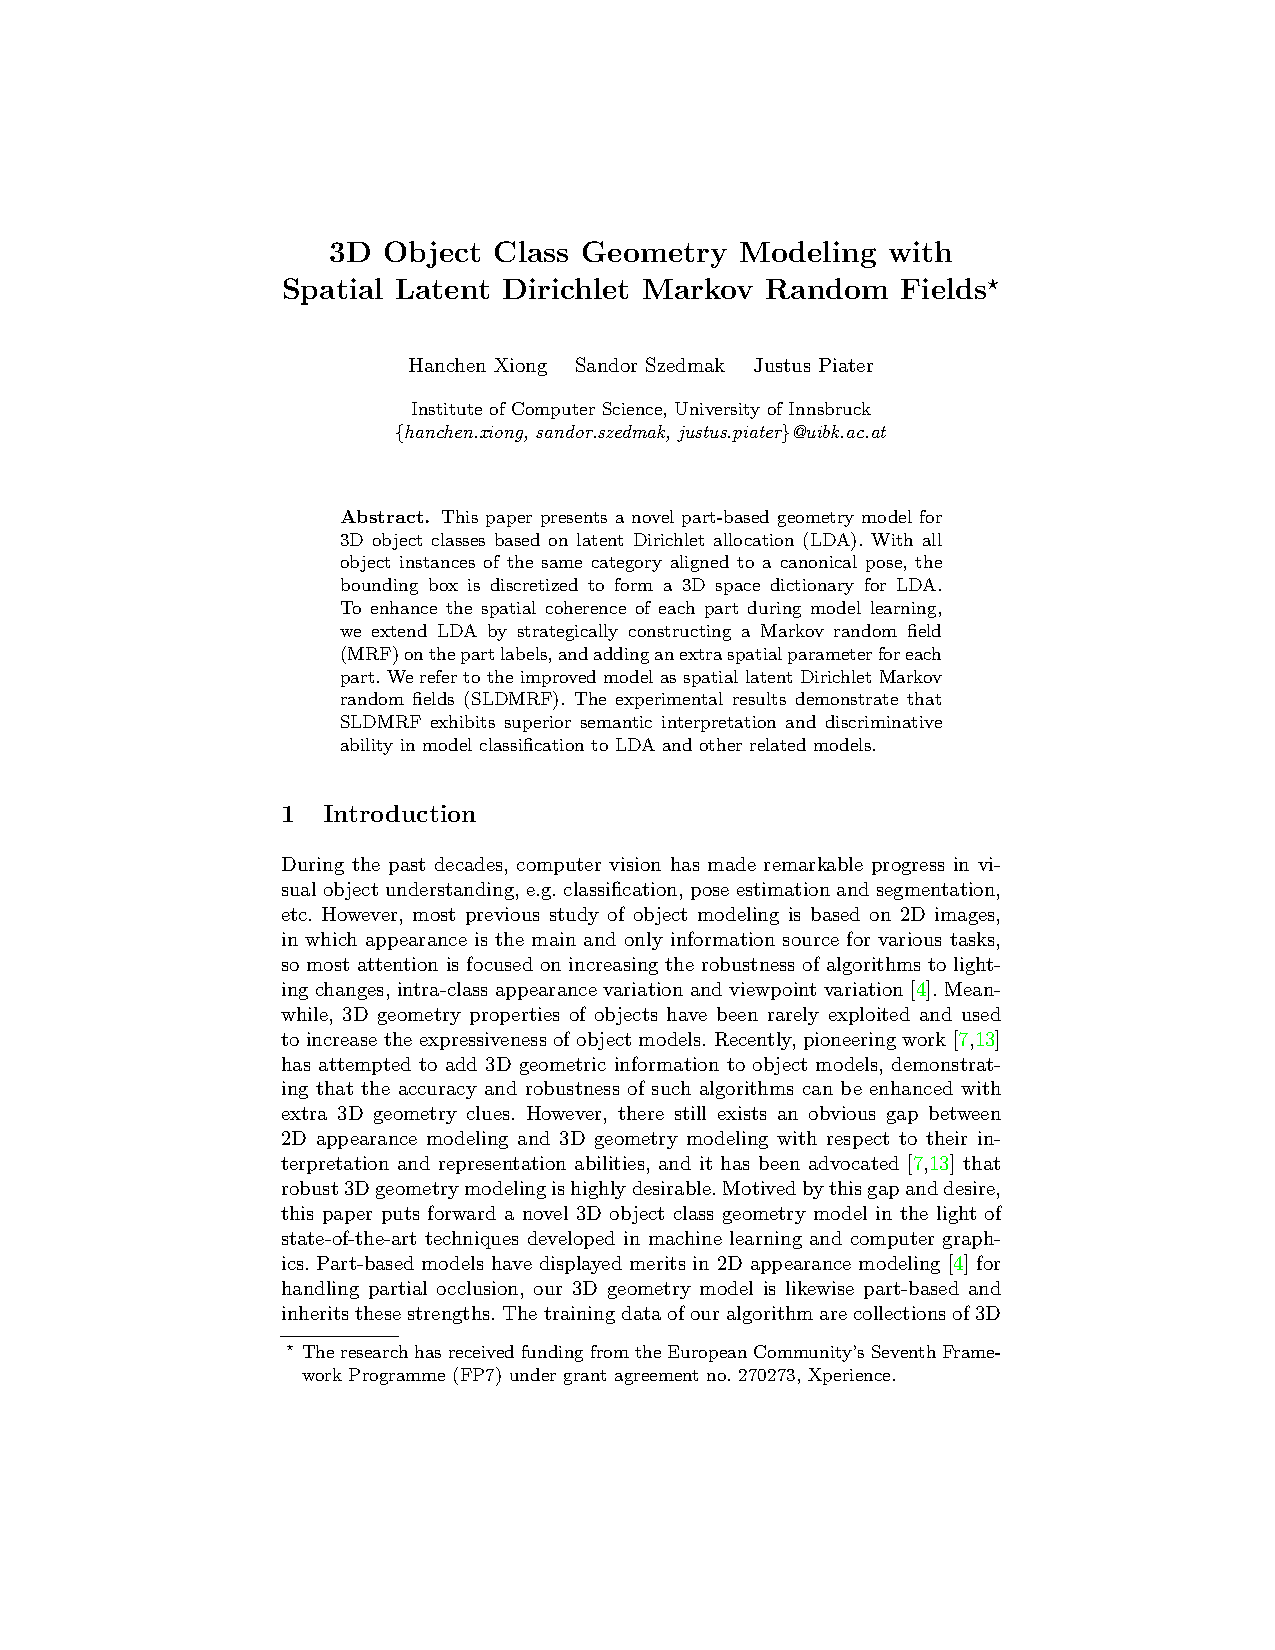
\includepdf[offset=3cm -2.5cm, scale=1.2, pages=-,pagecommand={\pagestyle{fancy}}]{./Papers/Xiong-2013-GCPR.pdf}
